\chapter{TeraSort与数据立方的结合}

TeraSort \cite{o2008terabyte} 最初的提出是用于在 MapReduce 中对全局数据的排序。\cite{tao2013minimal} 提出了 TeraSort 最佳的采样比例,并证明了该比例的合理性。该论文同时将 TeraSort 与 GroupBy 结合,提高在倾斜数据集况下 GroupBy 的计算效率。由于 GroupBy 是数据立方的子操作,因此受到这篇论文的启发,考虑将TeraSort与数据立方相结合。

\section{TeraSort}

TeraSort最初用于在 MapReduce 中对全局数据的排序。虽然 MapReduce 输出的最终结果是有序的,但仅是每个 reducer 输出的数据是有序的,而 reducer 之间的数据是无序的。图\ref{tera_sort}为不使用 TeraSort 与使用 TeraSort 的情况下对原数据使用 MapReduce 排序的结果。图中每个矩形内的数据表示 每个 reducer 的输出。对于不使用 TeraSort 的MapReduce,每个 reducer 输出的数据都是有序的,但是reducer 之间的数据是无序的。而对于使用 TeraSort 的 MapReduce,不仅仅是每个 reducer 内的数据是有序的,reducer 之间的数据也是有序的。

\begin{figure}[ht] 
\centering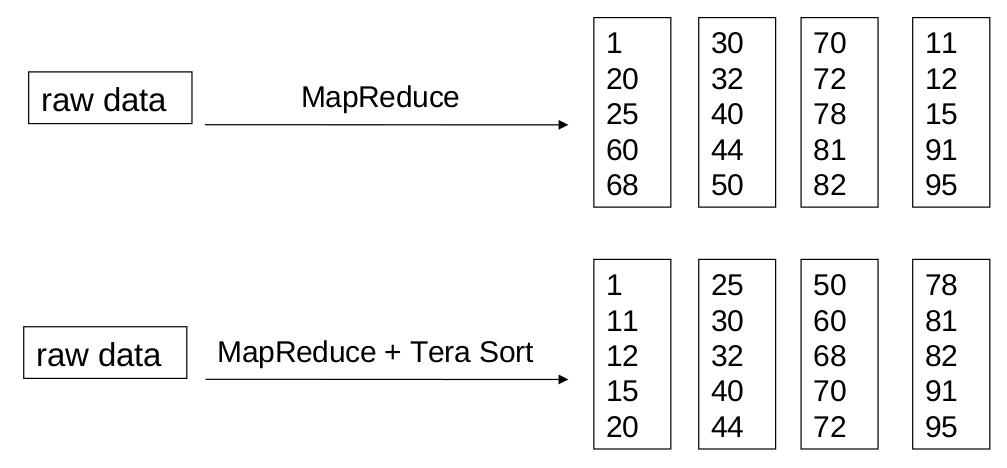
\includegraphics[width=4.5in]{picture/ch_terasort_mr/tera_sort} 
\caption{Tera Sort}\label{tera_sort} 
\end{figure}

TeraSort 能令全局有序的重要关键是,控制落到每个 reducer 上的数据的数据范围。也就是规定某一个范围内的数据必须落在指定的 reducer 上,而不是使用 MapReduce 本身的哈希函数将这些数据随机分发到各个 reducer 上。但如何确定这些范围值与 reducer 之间的关系呢,尤其是对原数据的数据特征并没有太多了解的情况下。这里使用采样的方法。

对原数据进行一定比例的采样,这个最佳比例 \cite{tao2013minimal} 已给出证明。接着将采样的数据都发到同q一个 reducer 上。根据 MapReduce 的特性,同一个 reducer 内的数据会被排序。若采样的样本大小为 s,reducer 的数量为 t。那么要从采样序列中选取 t-1 个点作为分界点,这些分界点是限定落入 reducer 中的数据的数据范围。对于第 i 个分界点选取的方法是,选取采样序列中的第 $i\times \left \lceil \frac{s}{t} \right \rceil$ 作为第 i 个分界点。图 \ref{tera_sort_mr1} 为  TeraSort 采样以及选取分界点的过程。图中假设 reducer 数据量为4,因此选取的分界点数量为3,红色的数字表示其被选为分界点。图中选取了3个分界点,分别为25、50、78,这就给出了4个 reducer 接收的数据范围,分别是$\left[- \infty, 25 \right], \left(25, 50 \right], \left(50, 78 \right], \left(78, +\infty \right]$。

\begin{figure}[!htb] 
\centering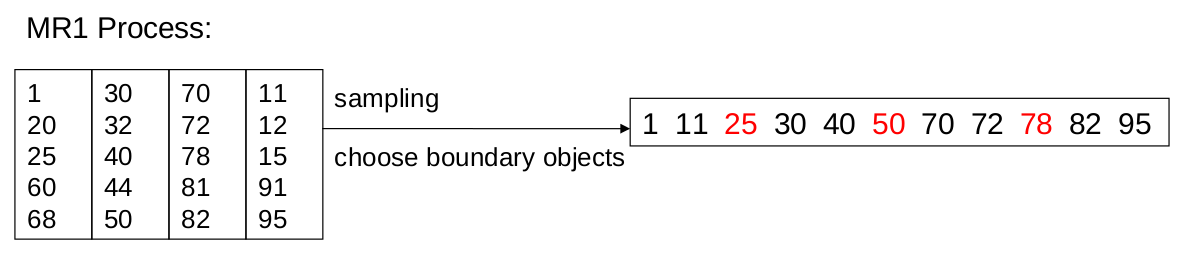
\includegraphics[width=6in]{picture/ch_terasort_mr/tera_sort_mr1} 
\caption{Tera Sort 采样与选取分界点}\label{tera_sort_mr1} 
\end{figure}

以上是第一轮 MapReduce,主要工作是采样以及选取分界点。这些分界点的作用是规定数据必须根据不同的范围落入既定的 reducer 上。在第二轮的 MapReduce 中,对于 Mapper 输出的每一条键值对,根据 key 的值,可使用二分查找等方法(Hadoop中使用Trie树)确定每一条键值对需要分发到的 reducer。最终 MapReduce 的结果就能全局有序。因此这里需要两轮 MapReduce。

\section{TeraSort与GroupBy}

\cite{tao2013minimal} 中将 TeraSort 与 GroupBy结合,能很好地解决倾斜数据集中由于各个 reducer 接收到的要计算的数据量差别过大,导致部分 reducer 运行时间过长的情况。

首先阐述使用 MapReduce 计算 GroupBy 的一般方法(称为Base GroupBy)。其实这个方法与 使用 MapReduce 计算数据立方的 Naive 方法类似。在 数据立方中,mapper的输出是每一条记录与所有 region 的映射。而在 GroupBy 中,仅需要与一个 region,即 GroupBy 的 region 映射即可。例如记录 e1=[a0, b0, c0, d0, m0],其中a0, b0, c0, d0对应的是维属性,m0 对应的是度量属性。当前操作是 GroupBy(B),那么对于这条记录输出的 key 为 b0,value 为 m0。具有相同的 key 值的数据会被分发到同一个 reducer 上计算,也就是具有相同 group\_value 的数据会被分发到同一个 reducer 上计算。如果数据集是倾斜的,也就是这个 region 内有一些特别大的 group,这将导致有一些 reducer 分发到大量的数据,而一些 reducer 分发到较少量的数据,导致最终计算效率的下降。

将 TeraSort 与 GroupBy结合,目的是将 region 内较大的 group 进行划分,从而将一个 group 分发到多个 reducer 上进行计算。而 TeraSort 的采样以及分界点的选择恰好能对大的 group 进行划分。论文中以度量函数 SUM 作为例子,采样的数据是维属性与记录编号组成的组合键。也就是采样的key是[group\_value, tuple\_id]这样的组合键。之后的操作与 TeraSort 类似,将采样的数据发到一个 reducer 上,采样的数据会被排序,然后根据 reducer 的数量选取分界点。由于这里的key是复合键,因此在 group\_value 相同的情况下会比较 tuple\_id。也正因为这个tuple\_id,较大的 group 才能被划分。

图 \ref{ts_groupby} 是使用 TeraSort 方法对采样的数据进行划分的示例。图中每个矩阵表示一个 group,矩阵越大,表示采样数据中具有相同 group\_value 的样本越多。红色的线表示分界点。分界点之间的间距是基本相同的,因此对于较大的 group 很有可能从中选取一个或多个分界点,正好将 group 进行了划分。若采样的key中只有 group\_value,而没有 tuple\_id,那么对于一个大 group,就算从中选择了多个分界点,但分界点的值都是相同的,这样的分界点就没有意义了。

图中每个分块都标有数字,各个分界点之间有多个分块,两个分界点之间的区域称之为分界区域。在同一个分界区域内的不同分块都会分派到同一个 reducer 上进行计算。但由于 group\_value 的不同,即使这些分块分到同一个 reducer 上,也会多次调用 reduce 函数。只有同一个 reducer 中具有相同 group\_value 的数据才会放在同一个 reduce 函数中进行计算。

\begin{figure}[!ht] 
\centering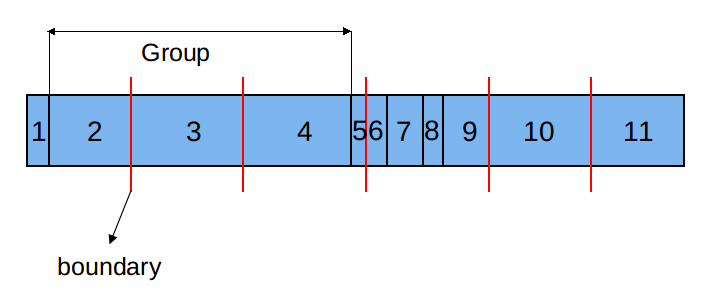
\includegraphics[width=4in]{picture/ch_terasort_mr/ts_groupby} 
\caption{使用TeraSort划分GroupBy的计算}\label{ts_groupby} 
\end{figure}

以上的采样以及选取分界点是第一轮的 MapReduce。第二轮的 MapReduce 与上面提到的计算 GroupBy 的一般方法类似,只是 key 的输出不仅仅是 group\_value,还需要tuple\_id。这样才能通过与分界点的比较确定数据要分发到某个确定的 reducer 上。使用 TeraSort 计算 GroupBy 还需要第三轮的 MapReduce,因为在上一轮的计算中,大的 group 被划分了,因此第三轮的 MapReduce 是对被划分的 group 进行合并。

\section{TeraSort与数据立方}

由于 GroupBy 是数据立方的一个子操作,受到 TeraSort 与 GroupBy 结合的启发,自然地引申到了 TeraSort 与数据立方的结合,并且发现这样的结合能解决上一章中提到的 MR-Cube 存在的一些问题。为了方便,以下将 TeraSort 与数据立方结合的方法称为 TS-Cube。

\subsection{数据采样与划分}

无论是 MR-Cube 还是 TS-Cube 都要解决一个问题,那就是大 group 的划分问题。在 MR-Cube 中是通过采样,然后根据采样数据中 group 的大小确定 region 是否为 reducer-unfriendly region。对于 reducer-unfriendly 的region,region 内的 group 都需要进行划分。MR-Cube 使用对某个属性值求余的方法对数据进行划分。对于 TS-Cube,运用 TeraSort 的思想,则同样需要采样,然后对采样数据排序,选取分界点。在 GroupBy 的场景下,采样的 key 是 [group\_value, tuple\_id] 这样的复合键,在数据立方的计算中,由于计算的不仅仅是一个 region,因此采样的 key 更为复杂。并且\cite{tao2013minimal} 中讨论的度量函数仅是 SUM,而这里还需要考虑到整体性度量函数。

首先考虑采样的 key 值。采样的 key 值关系到分界点的选取以及第二轮 MapReduce 计算时 reducer 中数据的均匀性。因为数据立方的计算涉及到多个 region,因此复合键中要加入与 region 有关的信息,这里选择加入 region\_id。将各个 region 按照字符串顺序排序,然后对它们编号,即可得到 region\_id。这样使用[region\_id, group\_value] 复合键即可表示一个指定 region 内指定的 group。但仅用这两个值对于大的group是无法划分的。因为若两个分界点落在同一个region的同一个group内,这两个分界点的值也是相同的,因此这里需要加入更多的信息。

在第二章准备知识中一共提到三种度量函数,这里可将这三种度量函数分为两类,一类是非整体性度量,另一类是整体性度量。以下分别阐述这两种不同的度量在采样时 key 值的构成。

对于非整体性度量,由于数据划分不受限制,因此数据不需要按照某个特定的属性进行划分。所以这里可以与选择 tuple\_id 作为 key 值的一部分。并且 tuple\_id 一般是数据的主键,主键是无重复的。这种情况下,一个 group 内若有多个分界点,分界点的值也是不同的。因此,对于非整体性度量函数,采样时的key为 [region\_id, group\_value, tuple\_id]。

而对于整体性度量,随意的数据划分对它的计算很可能是无任何帮助的。在这里,可使用 \cite{nandi2011distributed} 提出的部分线性度量(Partially Algebraic Measure)。也就是根据不同的整体性度量函数按照某个特定的属性值进行划分,而这个属性值在多数情况下都是度量属性值。因此,对于整体性度量函数,采样时的key为 [region\_id, group\_value, measure\_value]。这种情况下,即使一个 group 内有多个分界点,因为度量值的不同,分界点的值也不同。

同时,这样的划分对于计算也是有一定帮助的。例如 COUNT(DISTINCT(uid)),uid 为度量值,那么采样的key为 [region\_id, group\_value, uid]。因此相同的 uid 必定会划分到同一个分块内,因此对于每个分块仍然可以计算 COUNT(DISTINCT(uid)),然后对每个分块的结果做累加即可。图\ref{tscube_picture} 为 TS-Cube 的采样与分界点的选取。每一个矩阵表示一个 group,相同颜色的矩阵表示同一个 region 内的 group。红色的直线表示分界点。从图中可看出分界点更容易落在较大的矩形上,也就是大的 group 更容易被划分,从而分派到多个 reducer 上进行计算。这里与 GroupBy 的情况也是类似的,虽然一个 reducer 中有多个分块,但是只有相同region\_id 和 group\_value 的数据才会在同一个 reduce 函数上进行计算。

\begin{figure}[!htb] 
\centering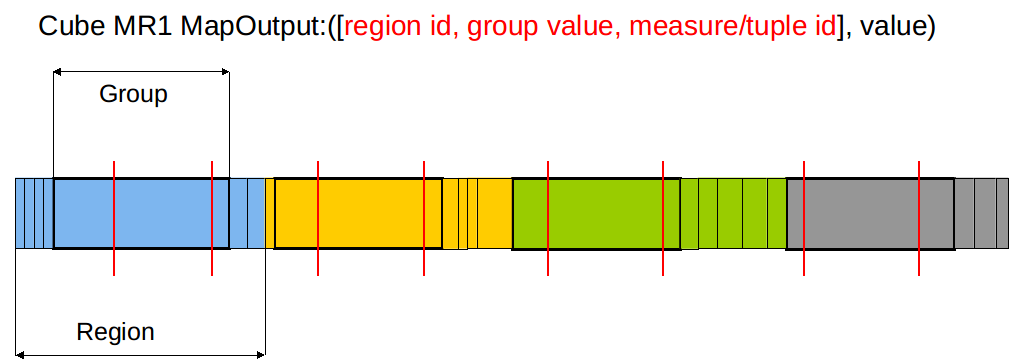
\includegraphics[width=6in]{picture/ch_terasort_mr/tscube_picture} 
\caption{TS-Cube的采样与分界点的选取}\label{tscube_picture} 
\end{figure}

根据以上的方法所选取的分界点即规定了每个 reducer 所要处理的数据范围。group 越大,采样中所占的比例也越大,那么分界点越容易落在其上。因此能达到大group被划分的目的。而对于分界点数量,若有 t 个reducer,则至少要选取 t-1 个分界点。但其实可以选择更多分界点,只要保持是 (t-1) 的倍数关系即可。但这个倍数到底如何选择,目前仍未有一个较好的结论。

使用 TeraSort 这样的采样与数据的划分方式正好可以解决 MR-Cube 中 group 的划分问题。在 MR-Cube 中,只要一个 region 内有一个大 group,那么这个 region 内所有的 group 都要被划分。而在 TS-Cube内,分界点一般只会落在较大的 group 上,即使不落在较大的 group 上,也只会落在两个小的 group 之间。因为 group 越小,采样中出现的数量也越少,那么分界点落在这个小 group 上的概率也就非常小了。只有分界点落到的 group 才会被划分,这样 TS-Cube 一般只会划分大的 group。因此 TS-Cube 就可以避免了 MR-Cube 中出现的不必要的划分。

在 MR-Cube 中使用求余的方式对数据进行划分,在一些极端情况下,可能数据会有倾斜性,导致划分后的数据依然有倾斜性。例如使用 MR-Cube 的方法计算的划分因子的结果是2,也就是令某个属性值对2求余从而达到数据划分的效果,而需要划分的属性值若大部分都是奇数,这样将导致数据划分的失效。而使用 TS-Cube 的方法则可以避免这种情况。即使所有的度量属性值都是奇数,TS-Cube 依然可以较为均匀地划分数据。因为 TS-Cube 对数据的划分是基于数据出现的频率,数据出现频率越高,越容易被划分,也正好达到了大数据需要划分的目的。

\subsection{数据立方的计算}

以上的采样与分界点的选取是第一轮的 MapReduce,也即是对数据的划分。第二轮进行的 MapReduce 是对数据立方的计算。这里先不考虑将多个 group 的数据放在同一个 reduce 函数里计算的情况(即MR-Cube 中提出的 Batch Area),仍采用 Naive 的方法,映射所有的region。TS-Cube 与 Batch Area 的结合将在下一节中阐述。

根据使用 TeraSort 对数据进行全局排序以及计算 GroupBy 可看出来,第二轮的 MapReduce 中 mapper 输出的 key 一般与采样的 mapper 所输出的 key 是一致的。因为第一轮 mapper 输出的key中的若干个会被选为分界点,第二轮mapper的输出必须与第一轮保持一致,才可以与分界点进行比较,从而决定键值对落到哪个 reducer 上。决定键值对被分派到哪个 reducer 是在 MapReduce 的 partition 阶段。因此 mapper 输出的 key 与分界点的比较也正是在 partition 阶段。

而在 reduce 阶段,同一个 reducer 内的数据,若具有相同 region\_id 和 group\_value 则会在同一个 reduce 函数内进行计算。此处 reducer 的计算与 Naive 是一样的,因此不再详细说明。


这里需要为 MapReduce 的机制进行一些说明。在默认的 MapReduce 中,只有相同的 key 值的数据才会放在同一个 reduce 函数中计算。而在 TS-Cube 第二轮 MapReduce 中 mapper 输出的 key 值为 [region\_id, group\_value, tuple\_id or measure\_id],是一个复合键。按照默认规定,必须这3个值都相同才能放在同一个 reduce 函数内计算。但其实MapReduce的框架为此提供了灵活的变化。用户可重载 GroupPartitioner 函数,此函数是定义在同一个 reducer 内,具有什么特征的数据会被放在同一个 reduce 函数中计算。由于TS-Cube 的特殊性,这里需要重载 GroupPartioner,规定只要 region\_id 和 group\_value 相同的数据即可放在同一个 reduce 函数内计算。

最后进行第三轮的 MapReduce,将被划分的数据进行合并。这里合并的方法非常简单,并且实验证明也是很高效的。合并的方法与 MapReduce 做单词统计是类似的,因为第二轮 MapReduce 输出的 key 是 region\_id 和 group\_value,输出的 value 是 measure\_value。因此在第三轮的 MapReduce 中,只要将第二轮输出的数据读入,对相同 region\_id 和 group\_value 的数据做一次合并即可,这个过程与单词统计是一样的。虽然上一轮将部分的 group 进行划分,但是这个划分的数量是有限,因此合并过程中,具有相同 region\_id 和 group\_value 的数据也并不多。


\section{TS-Cube 与 Pipesort}

上一节中主要阐述了数据的划分,而在这一节中将详细阐述如何将多个 group 放在同一个 reduce 函数里计算,也就是减少数据立方计算过程中,中间数据的产生。 MR-Cube 提出了 Batch Area 的概念和一些划分 Batch Area 建议遵循的规则,但是并没有给出简单且具体的划分方法。同时 MR-Cube 中使用的是 BUC 对Batch 内的 group 进行计算,但其实这种方法并没有充分利用 MapReduce 框架的特点与优势。因此接下来是针对以上两点进行改进。


\subsection{PipeSort}

PipeSort\cite{agarwal1996computation} 是 1996 年由 Agrarwal 等人提出的一种计算数据立方的方法。Pipe 指的是 Pipeline,即流水线。它是一种自顶向下的计算数据立方的方法。它利用多个 group 之间具有共同前缀的特性,对数据只扫描一遍即可计算多个 group 的聚合。

如图\ref{pipesort} 所示,这是一个4维的数据立方其中一种可行的 pipesort 方案。每个虚线框内表示的是一个pipeline。这些 pipeline 之间是共享共同前缀的,例如 ABCD-\textgreater ABC-\textgreater AB-\textgreater A 这样一个pipeline,将数据按照 ABCD 这样的属性顺序排序,再对数据进行扫描,在扫描的过程中可同时计算 ABC、AB、A 的聚合。因为数据已经按照 ABCD 这样的维属性进行排序,那么具有相同 ABC、AB 或者 A 值的数据在顺序上必定会相连的,因此可通过一遍扫描计算出这 4 个 group 的聚合。

\begin{figure}[!htb]
\centering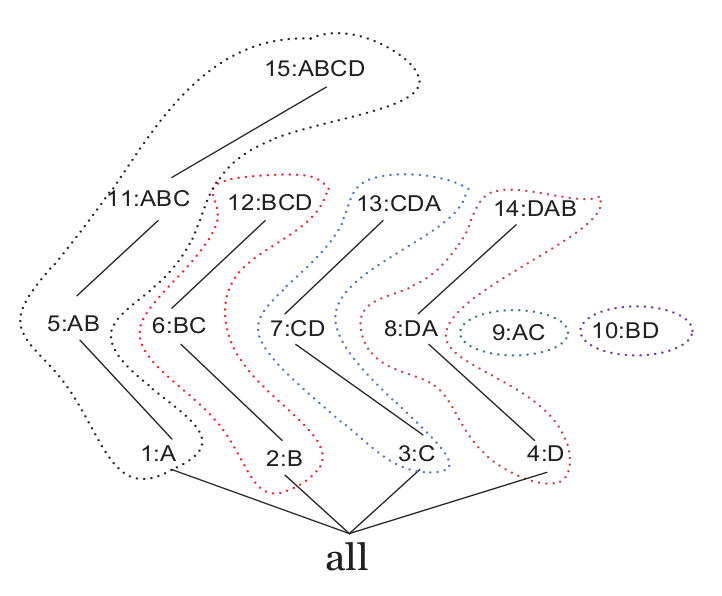
\includegraphics[width=3in]{picture/ch_terasort_mr/pipesort} 
\caption{4维数据立方的划分}\label{pipesort} 
\end{figure} 

正是因为 pipesort 的有序性以及一次性扫描的特点,它更适合应用于 MapReduce 的框架下。因为 MapReduce 默认对数据进行排序,无论用户是否需要,它都会对数据进行排序。用户还可以根据需要重载函数,自行定义排序时的比较函数。因此不需要额外地再对数据进行排序。其次,reducer 中提供的迭代器仅能够对数据扫描一次,若需要对数据进行多次扫描,则需要先将数据载入内存中。而 BUC 的正是需要多数据进行多次扫描,相反,Pipesort 仅需要对数据扫描一次即可,不需要额外的内存。BUC 更适合使用的场景是有条件限制的聚合操作,例如 HAVING。而对于无条件限制的情况下,Pipesort比BUC更适合在 MapReduce 中使用。

在 \cite{agarwal1996computation} 中,pipeline 方案是通过二分图匹配的方式得到。二分图匹配的方式是可以得到一个最优解,但它需要首先对数据采样从而估算各个 region 的大小,再使用二分图匹配的方法一层层地计算 pipeline 的方案。若在单机版且内存不足的情况下,这样的方案是非常有效的。但是当前论文研究的环境是分布式,计算资源和内存都是相对较充足的,并且结合上一节提到的数据划分方法,pipeline 方案的形成可以更简单。

在\cite{wang2013scalable} 中提出了使用随机贪心的方式形成 pipeline 方案。将所有的 region 都放入一个集合内,每次从集合中选择维度数量最多的一个 region。对region内的维度进行组合,对于每个组合都可以得到一种 pipeline 方案。选择一种pipeline 中 region 在集合中数量最多的方案。并且把该pipeline 中的region都从集合中移除。然后继续从集合中选择维度数量最多的region至集合为空。

例如对于 4 维的数据,维属性为ABCD。则在一开始选择维度数量最多的的 region,ABCD,它有多种组合,例如ACBD,ADBC等等,对于组合ABCD,可得到pipeline ABCD-\textgreater ABC-\textgreater AB-\textgreater A。这个pipeline中所有的region都在集合中,因此这个pipeline可选,并且把ABCD,ABC,AB,A这4个region从集合中移除。接着继续从集合中选择 region,假设选择了ACD,它有多种组合,例如ADC,CDA。对于ADC这个组合的pipeline是  ADC-\textgreater AD-\textgreater A,其中region A已经不在集合中,因此只有2个region在集合中。而对于CDA这个组合的pipeline是  DCA-\textgreater DC-\textgreater D,3个region都在集合中,因此选择 CDA 这个组合以及对应的pipeline。以此往下只集合为空。图\ref{pipesort} 是其中一种 pipesort 方案。

上述的方法比起二分图匹配更简单,虽然pipeline的方案不一定是最优的,并且pipeline之间的长度有一定的差距,但是由于计算资源与内存的充足,可以弥补到以上两点不足。并且将这种方法与上一节中的数据划分结合,一些大的group必然会被划分,就可令各个reducer的计算相对均匀。

但以上的方法若用于层次型的数据,则会导致pipeline之间的长度差别过大,尤其是在层次型较深或者各个层次数量差别过大的情况,因此这里对层次型数据生成 pipeline 的方法有所改动。以下继续沿用图 \ref{dataset_table} 作为数据集进行说明。该数据集的 lattice 如图\ref{dataset_lattice} 所示。



\begin{figure}[!htb]
\centering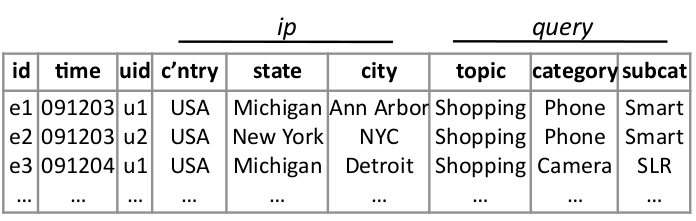
\includegraphics[width=3.5in]{picture/ch_datacube_mr/dataset_table} 
\caption{层次型数据集的表结构}\label{dataset_table} 
\end{figure} 

\begin{figure}[!htb]
\centering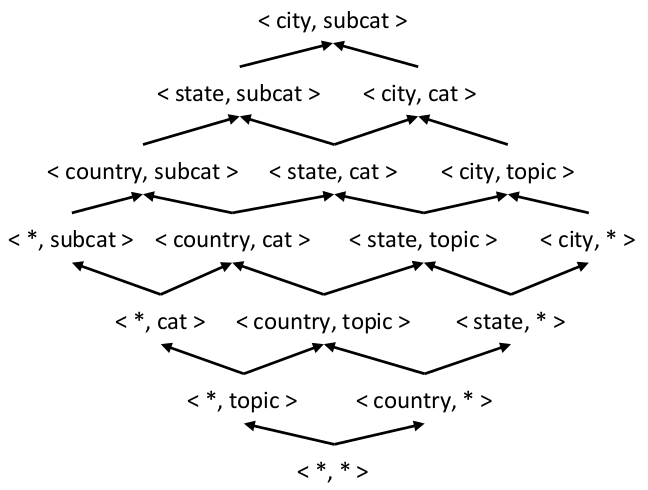
\includegraphics[width=3in]{picture/ch_datacube_mr/dataset_lattice} 
\caption{层次型数据集的lattice}\label{dataset_lattice} 
\end{figure} 

在该数据集中,共有6个维属性,分别为 country, state, city, topic, category, subcategory。其中 [country, state, city] [topic, category, subcategory] 是分别具有层次性的。将这6个属性从0开始编号,则如表\ref{attribute_no}所示。

\begin{table}[!ht]
\begin{center}
\begin{tabular}{|c|c|c|c|c|c|}
\hline 
Country & State & City & Topic & Category & Subcategory \\ 
\hline 
0 & 1 & 2 & 3 & 4 & 5 \\ 
\hline 
\end{tabular} 
\end{center}
\caption{数据集属性编号}\label{attribute_no}
\end{table}

对属性编号后,lattice 中的各个 region 可用编号组成的字符串表示。如 region \textless state, category \textgreater 可用字符串 ``0 1 * 3 4 *" 表示。又如 region \textless country, subcategory\textgreater 可用字符串 ``0 * * 3 4 5"表示。即对于要进行 GroupBy 的维属性在字符串中以编号出现,其他维属性则以 * 出现。由于数据集具有层次性,因此不可忽略该属性的前置属性。即 GroupBy(city) 时,默认等于 GroupBy(country, state, city),因此字符串中要出现 country 与 state。图 \ref{sorted_region}(a) 是将 lattcie 转化成字符串并按字典顺序排序后的结果。这里省略\textless *,* \textgreater 这个region。因为这个region只有一个 group 且涉及全部的数据,更建议单独计算,效率更高。对字符串排序后的结果发现这样的顺序正好有 pipesort 的特性!每4个字符串就刚好构成一个pipeline。\ref{sorted_region}(b)中每个红色方框表示一个pipeline。

\begin{figure}[!ht] 
\centering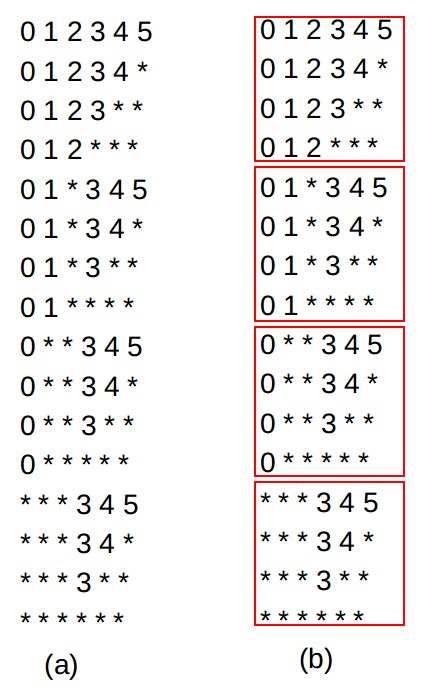
\includegraphics[width=2in]{picture/ch_terasort_mr/sorted_region} 
\caption{按字符串顺序排序的Region}\label{sorted_region} 
\end{figure}

这样的一种将region转化成字符串再排序的方法,对于层次型的数据集非常适用,因为它们具有层次型特征,在对字符串排序后,根据排序结果能直接形成 pipeline 。由于数据集的层次是既定的,因此形成的每个 pipeline 之间的 region 的数量基本是相等的,这样每个 reducer 要计算的 region 也是相对平均的。

因此这里建议,对于非层次性的数据集可使用 \cite{wang2013scalable} 中的方法形成 pipeline 方案,而对于层次性的数据集则使用region转换成字符串排序后形成的pipeline 方案。

\subsection{TS-Cube 与 PipeSort 的结合}

最后将 TS-Cube 与 pipesort 结合,从这两个方面一同提高数据立方的计算效率。TS-Cube 可对大的group 进行划分,pipesort 可减少中间数据的产生,并且将多个 group 放在同一个 reduce 函数中计算。由于 pipesort 的使用,无论是采样还是数据立方的计算,mapper 的输出不再是映射所有的 region,而仅需要映射这个pipeline 中的一个 region 即可。下面以 ABCD-\textgreater ABC-\textgreater AB-\textgreater A 这个pipeline,e1=[a0, b0, c0, d0, m0]这条记录为例,分别分析采样与数据立方计算时 mapper 的输出。

在TS-Cube 的第一轮 MapReduce中,mapper 输出的样本的 key值应为[region\_id, group\_value, tuple\_id or measure\_value]。这里对应上述的pipeline 和记录,mapper 输出的key应为 [Region(A)\_id, a0, tuple\_id or measure\_value]。

在TS-Cube 的第二轮 MapReduce 中,mapper 输出的key应与第一轮是一致的,因此mapper 输出的key为[Region(A)\_id, a0, tuple\_id or measure\_value],输出的value则为[b0, c0, d0] 这样的组合键。在上面的章节中提到,MapReduce的机制较为灵活,可重载 GroupComparator 函数,令只要有相同 region\_id 和 group\_value 的数据都放在同一个 reduce 函数中。因此在同一个 reducer 中,对于属性 A 具有相同值的数据都会放在同一个 reduce 函数里,即使它们的 tuple\_id 或 measure\_value 不同。

由于 pipesort 的使用,mapper 的输出不再是映射所有的 region,而仅需要映射 pipeline 中的一个 region 即可,而在这里 mapper 的key值选择了 region(A) 作为映射,而将剩余属性的值放在了value中。若在单机上使用 pipeline 计算数据立方,只要将数据按照 ABCD 这样的属性顺序排序,然后对数据扫描一遍即可计算 GroupBy(ABCD),GroupBy(ABC),GroupBy(AB),GroupBy(A)的值。但是在分布式中,需要对数据进行划分,而我们希望数据的划分能在满足 pipeline 计算的同时每个分块尽可能地小。这样可减轻 reducer 在shuffle 和 sort 阶段的负担,提高计算效率。为了满足 ABCD-\textgreater ABC-\textgreater AB-\textgreater A 这个 pipeline 的计算,具有相同属性 A 的值的数据必定要放在同一个分块内(除非由于这个 group 过大,被分界点划分了)。那么数据则根据属性A的值被分成若干个分块,每个分块上都可进行 pipeline 的计算,并且互相是不影响的,从而实现了多个pipeline的并行计算。

对于任何一条 pipeline,起始的region 一定是属性数量最多的,末尾的reigon一定是属性数量最少的。对于每条记录,都要与每个pipeline做映射。在数据立方的计算中,mapper 输出的 key值为 末尾region对应的属性值与tuple\_id 或 measure\_id的组合,mapper 输出的value 值为起始region中的属性除去 末尾region的属性后对应的属性值。如图\ref{dataset_table} 对应的数据集,生成的pipesort方案如图\ref{sorted_region}所示共有4个pipeline,因此每条记录都要映射4个键值对。

\subsection{实现伪代码}

{\renewcommand\baselinestretch{1} 

\begin{algorithm}
\caption{Naive Algorithm}

{%\fontfamily{ptm}\selectfont

	\begin{algorithmic}[1] %每行显示行号
    \Function {MAP}{e}
    	\State e is a tuple in the dataset
        \ForAll {Region R in C}
        	\State k=R(e)
        	\State EMIT(k, e)
        \EndFor
   	 \EndFunction
     \State
     \Function {REDUCE}{k,{e1,e2,...}}
     	\State let M be measure function
        \State EMIT(k, M({e1,e2,...}))
     \EndFunction
	\end{algorithmic}

}

\end{algorithm}

\par}

\section{TSP-Cube 与 MR-Cube的比较}









